\documentclass[final,hyperref={pdfpagelabels=false}]{beamer}
\usepackage{grffile}
\mode<presentation>
  {
  %  \usetheme{Berlin}
  \usetheme{I6pd2}
  }
  \usepackage{times}
  \usepackage{amsmath,amsthm, amssymb, latexsym}
  \boldmath
  \usepackage[english]{babel}
  \usepackage[latin1]{inputenc}
  \usepackage[orientation=portrait,size=custom,width=80,height=120,scale=1.4]{beamerposter}  
  
  % my packages
  
  %%%%%%%%%%%%%%%%%%%%%%%%%%%%%%%%%%%%%%%%%%%%%%%%%%%%%%%%%%%%%%%%%%%%%%%%%%%%%%%%%5
  \graphicspath{{figures/}}
  \title{Optimizing Simulink\textsuperscript{\textregistered} Diagrams}
  
  \author{Bentley James Oakes}
  
  \institute[McGill University]{McGill University, Montreal, Canada}
  
  \date{\today}


  %%%%%%%%%%%%%%%%%%%%%%%%%%%%%%%%%%%%%%%%%%%%%%%%%%%%%%%%%%%%%%%%%%%%%%%%%%%%%%%%%5
  \begin{document}
  \begin{frame}{} 
  \vspace{-1.8cm}
      \begin{columns}[t]
        \begin{column}{.993\linewidth}
        \begin{block}{\large Problem Statement}
        \small
   		The Simulink\textsuperscript{\textregistered} modelling tool is used to diagram and study cyber-physical systems. One advantage
   		of modelling the systems in this way is that embeddable code can generated from the models directly.
   		However, this process means that inefficiencies in the model may be propagated to the code. Code
   		generation optimizations are available, but may lead to an unacceptable loss of traceability in determining
   		which parts of the model were modified or removed during code generation.\\~\\
   	    Our works focuses on defining model-to-model optimizations. This means that the optimized
   		model can be loaded back into Simulink for further development or analysis, improving traceability and
   		allowing model specialization for different platforms. An analysis framework has been created, based on
   		dataflow analysis from the compiler optimization domain. This allows fast and accurate definition of new
   		optimizations. As well, an initial optimization classification was developed to aid in the discovery of new
   		optimizations.
        \end{block}
        \end{column}
      \end{columns}         

    \begin{block}{Optimization Classification}
    \begin{center}
    \small
    In our work, we propose a classification for causal-block model optimization, based upon the platform-dependence and intent of the optimization. We believe that defining classifications for optimizations will create
    stronger theoretical connections to the compiler domain, as well as to transformations from the model
    transformation field.
    \end{center}
    \vspace{-1.5cm}
            \begin{columns}[t]
             \begin{column}{.19\linewidth}
           \begin{center}\textbf{Model-level}\end{center}
           \footnotesize
           The model-level optimizations are those that are not dependent in any way on the target architecture, and focus on changing the structure itself of the model. \\~\\Examples include, dead-block removal where
           blocks that are not needed for calculation in the system should be removed, or algebraic simplification of models to reduce computational effort.
           \end{column}
           \hspace{-1.2cm}\vrule\hspace{.05cm}
           \begin{column}{.19\linewidth}
          \begin{center}\textbf{Platform-independent}\end{center}
          \footnotesize
            In this second level of optimization generality, optimizations are specific to a general class
            of target architecture, such as whether the target is single- or multi- core, or the
            target programming language of code generation. \\~\\Example optimizations include transforming
            floating point calculations into integer representations, and specializing blocks into structures appropriate for a given
            target language.
            \end{column}
            \hspace{-1.2cm}\vrule\hspace{.05cm}
            \begin{column}{.16\linewidth}
          \begin{center}\textbf{Platform-dependent}\end{center}
          \footnotesize
            Platform-dependent optimizations can be characterized by their dependence on a particular target
            architecture. \\~\\Examples include rearranging the model in order to take advantage of a particular machine's
            caching strategy or hardware layout.
            \end{column}
            \hspace{-1.2cm}\vrule\hspace{.05cm}
            \begin{column}{.18\linewidth}
          \begin{center}\textbf{Optimization Hierarchy}\end{center}
          \footnotesize
            These classification levels can be placed in a hierarchical relationship, with optimizations
            further down the hierarchy more specific to a particular machine. \\~\\A code synthesis workflow may include transformations between these levels, so that a general model is specialized further and further until code is generated from a platform-specific model.
            \end{column}
            
            \begin{column}{.20\linewidth}
          ~\\~\\
            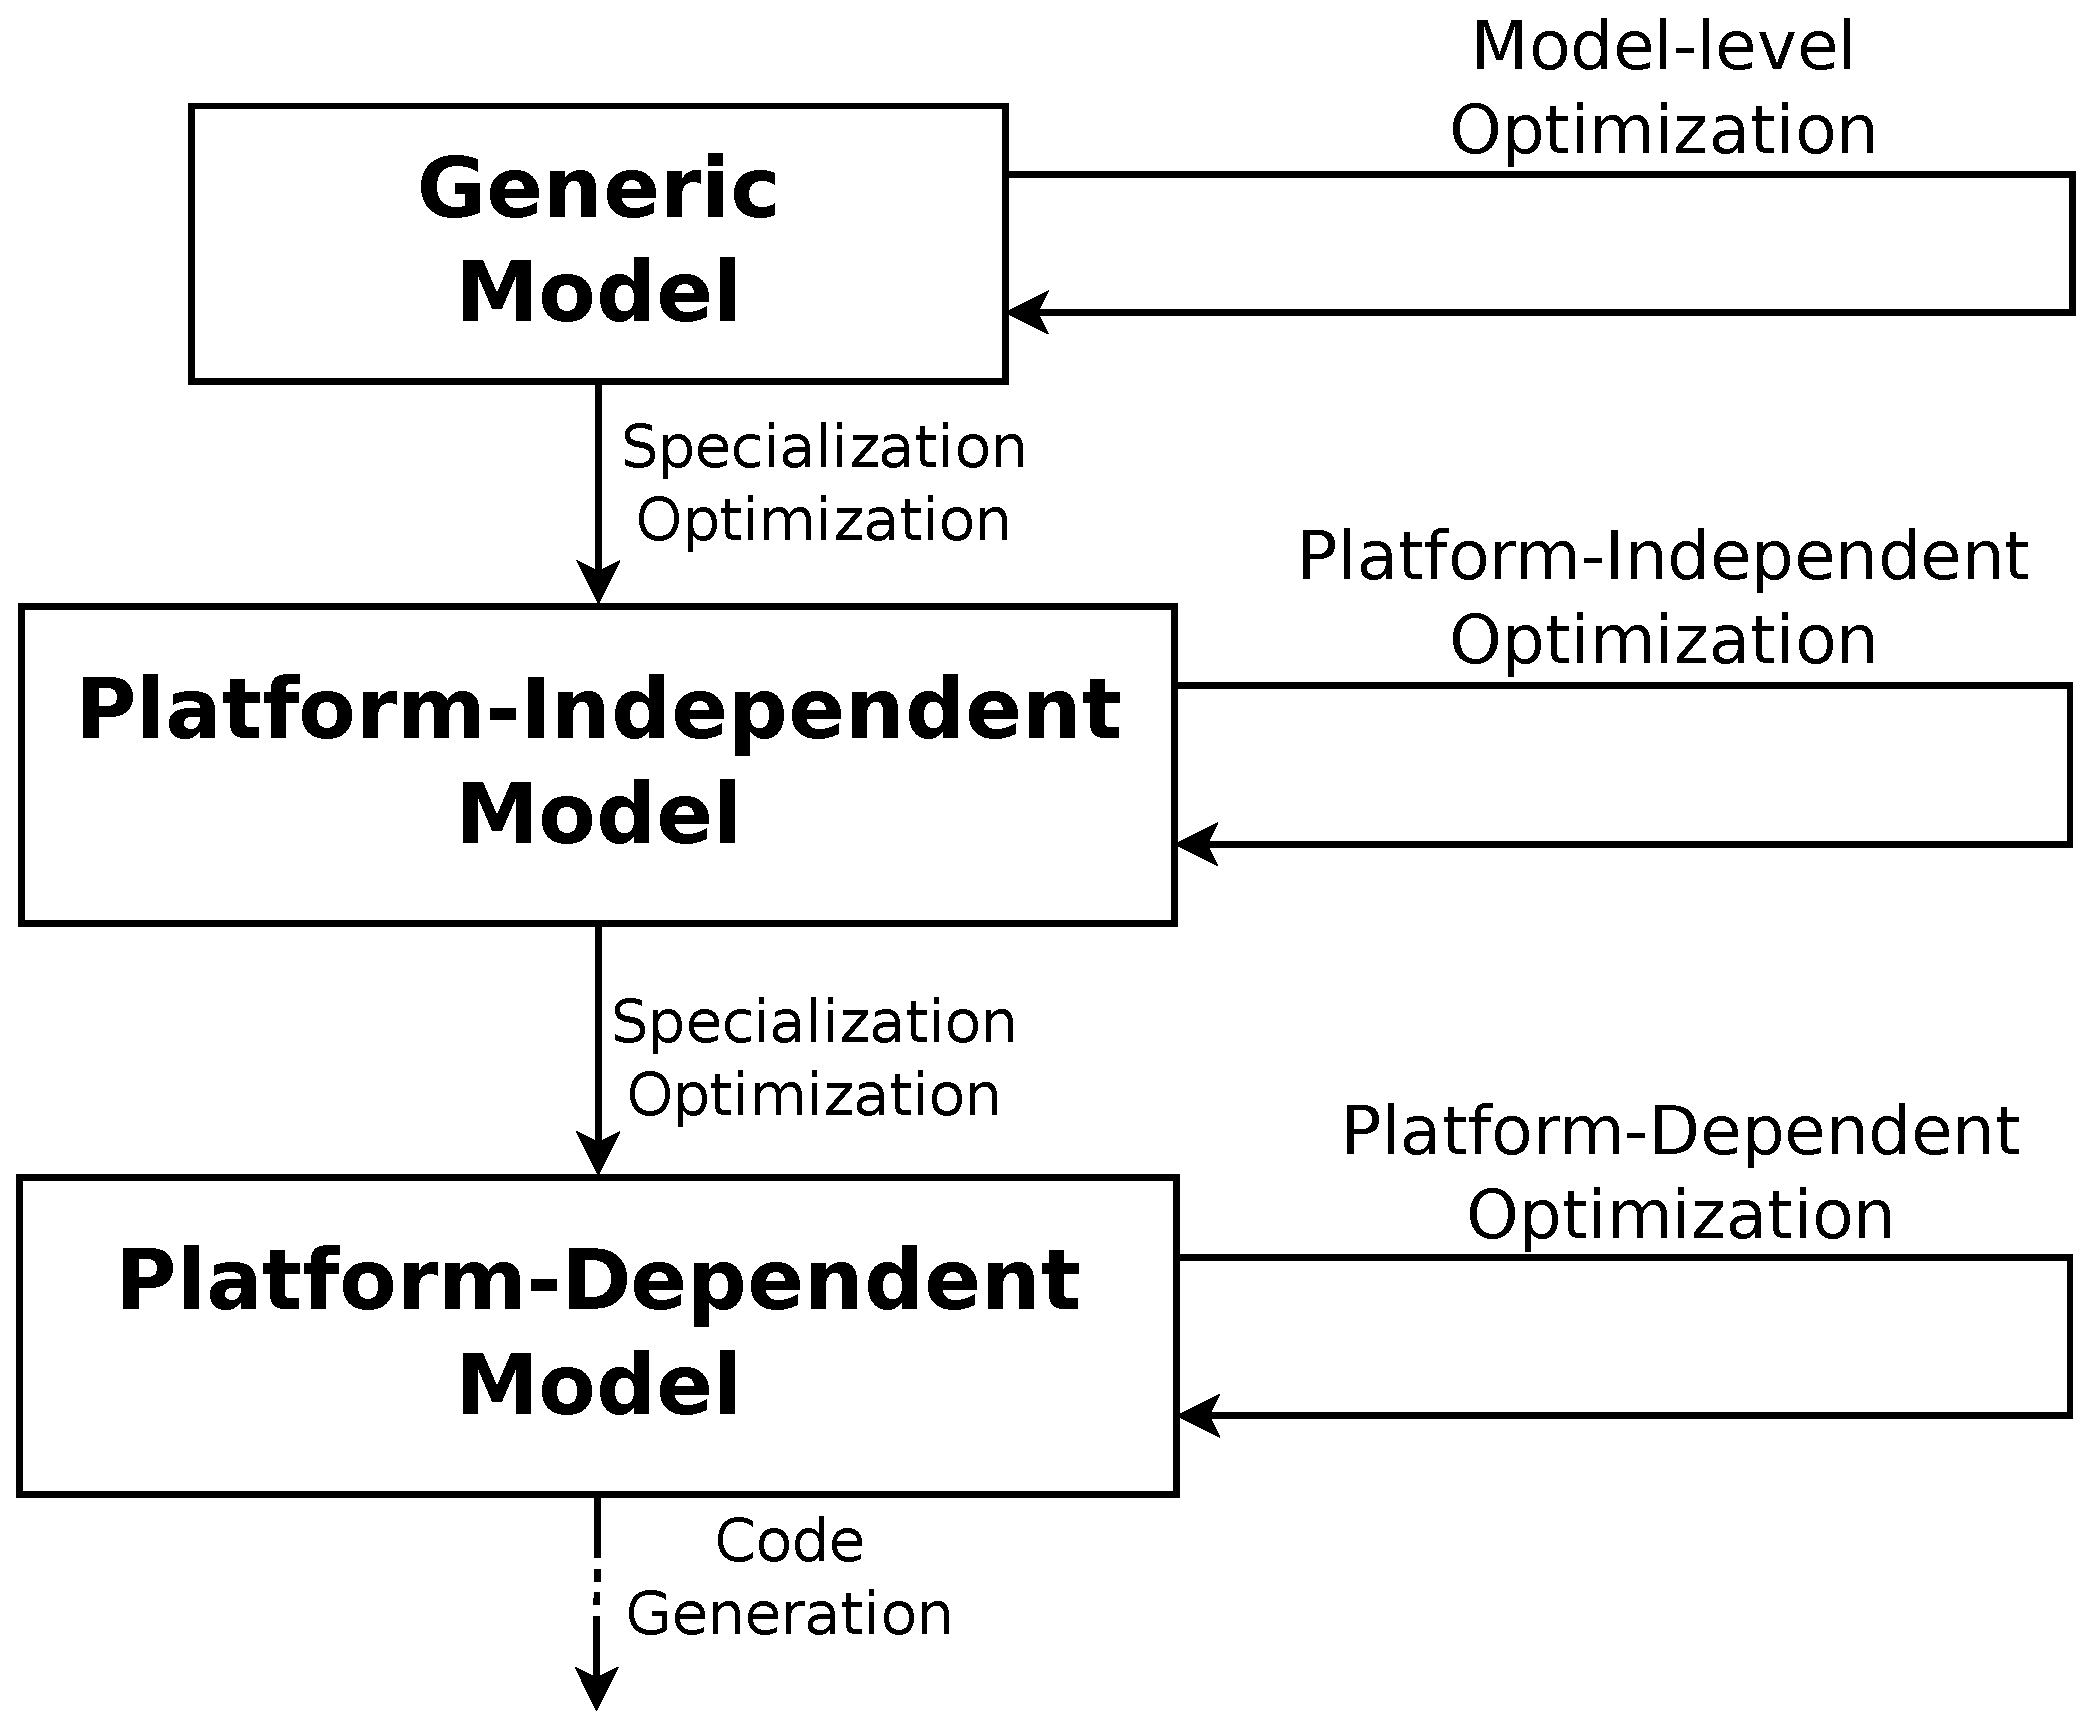
\includegraphics[width=\textwidth]{images/hierarchy}
            \end{column}
                        
                  \end{columns}
            \end{block}
	
        \begin{block}{Optimization Procedure}
        \vspace{-1.5cm}
        \begin{columns}[t]
         \begin{column}{.485\linewidth}
         \vspace{-.8cm}
       \begin{center}\textbf{Analysis}\end{center}
       \footnotesize
       Our work defines an analysis procedure to collect dataflow information for each node in the Simulink model. This procedure is based upon that used in the compiler literature. For example, for constant folding, the information propagated is whether a block will always produce a constant value during simulation.
       \end{column}
       \begin{column}{.485\linewidth}
       \vspace{-.8cm}
      \begin{center}\textbf{Transformation}\end{center}
        \footnotesize
        The optimization framework can then transform the model, based on the analysis results. This transformation is performed by utilizing the Himesis model format. After the transformation is complete, the optimized model is imported back into Simulink. This provides a second model to be further tested or modified.
        \end{column}
              \end{columns}
        \end{block}
      
      \vspace{-1.5cm}
    \begin{columns}[t]
    \centering
      \begin{column}{.585\linewidth}
        \begin{block}{Example Optimizations}
         \vspace{-.8cm}
        \small
        \begin{center}\textbf{Constant Folding}\end{center}
        
        \begin{columns}[c]
        \begin{column}{.485\linewidth}
        \begin{center}
        
        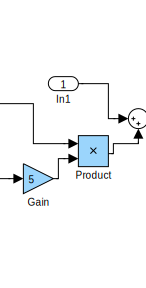
\includegraphics[width=0.8\linewidth]{images/models/Const1}\\
        \footnotesize Model before
        \end{center}
        \end{column}
        \begin{column}{.485\linewidth}
        \begin{center}
        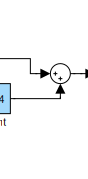
\includegraphics[width=0.8\linewidth]{images/models/Const1_export}\\
        \footnotesize Model after
        \end{center}
        \end{column}
        \end{columns}
        \footnotesize ~\\
        The constant folding optimization determines which blocks will always produce a constant value. For example, the four blocks on the left in the original model can be replaced by one constant block. This reduces the computation effort required by this model.
         ~\\~\\
         \hrule
         \small
          \begin{center}\textbf{Dead-Block Removal}\end{center}
                 
         \begin{columns}[c]
         \begin{column}{.485\linewidth}
         \begin{center}
         
         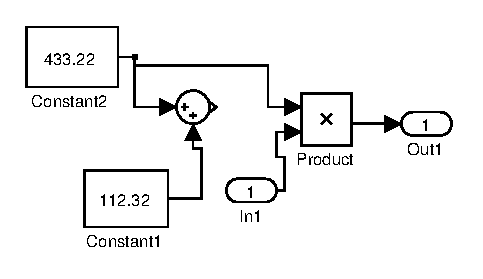
\includegraphics[width=0.8\linewidth]{images/models/HSimpleConstDead}\\
          \footnotesize Model before
         \end{center}
         \end{column}
         \begin{column}{.485\linewidth}
         \begin{center}
         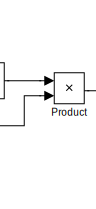
\includegraphics[width=0.8\linewidth]{images/models/HSimpleConstDead_export}\\
        \footnotesize Model after
         \end{center}
         \end{column}
         \end{columns}
          \footnotesize ~\\
         The constant folding optimization determines which blocks will always produce a constant value. For example, the four blocks on the left in the original model can be replaced by one constant block. This reduces the computation effort required by this model.
          ~\\~\\
         \hrule
          \begin{center}\textbf{Flattening}\end{center}
                 
         \begin{columns}[c]
         \begin{column}{.485\linewidth}
         \begin{center}
         
         
\includegraphics[width=\linewidth]{images/models/Flatten1}\\
         Blah blah blah
         \end{center}
         \end{column}
         \begin{column}{.485\linewidth}
         \begin{center}
         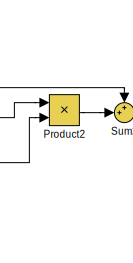
\includegraphics[width=\linewidth]{images/models/Flatten1_subsystem}\\
         Blah blah blah
         \end{center}
         \end{column}
         \end{columns}
         \begin{center}
          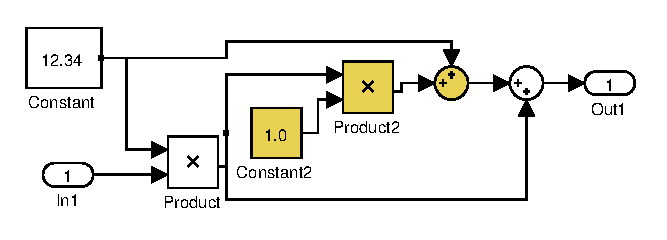
\includegraphics[width=\linewidth]{images/models/Flatten1_export}\\
          Blah blah blah
          \end{center}
         
        \end{block}
      \end{column}

     \begin{column}{.385\linewidth}
             \begin{block}{Experiments}
             \footnotesize
             \begin{table}[h]
             
             \centering
             \begin{tabular}{l | c c }
             
             \textbf{Experiment Step} & \textbf{Avg. Time (sec.)} & \textbf{Std. Dev.} \\\hline
              
             Connect to Simulink & 11.71 & .24 \\
             Import from Simulink & 4.94 & .04 \\
             Create model in Python & .08 & .01 \\
             Analysis & .02 & .00 \\
             Transformation & .01 & .00 \\
             Export to Simulink & .01 & .01 \\
             
             
             \end{tabular}
             ~\\~\\
             \footnotesize \textit{Representative timings for performing an optimization}
             \end{table}
             
             \begin{table}[h]
             
             \centering
             \begin{tabular}{l | c c c c }
             
             \textbf{Optimization} &\multicolumn{2}{c}{\textbf{Original Model (sec.)}}& \multicolumn{2}{c}{\textbf{Transformed Model (sec.)}} \\
              & \textbf{Avg.} & \textbf{Std. Dev.} & \textbf{Avg.} &\textbf{ Std. Dev.}\\\hline
              
             \textit{Constant Folding} & & & & \\
             Model 1 & \textbf{19.78} &.05 & \textbf{16.95} & .21\\
             Model 2 & \textbf{18.35} & .07 &\textbf{ 15.89} & .13\\
             Model 3 &\textbf{ 23.53} & .09 & \textbf{20.77} & .09\\
             Model 4 & \textbf{18.01} & .09 & \textbf{17.22} & .23\\
              & & & & \\
             \textit{Dead-Block Removal} & & & & \\
             Model 1 & 16.79 & .27 & 16.91 & .25\\
              & & & & \\
             \textit{Flattening} & & & & \\
             Model 1 & 18.87 & .22 & 18.75 & .19\\
             Model 2 & 21.77 & .16 & 21.75 & .38\\
             Model 3 & 19.54 & .12 & 19.94 & .06\\
             
             \end{tabular}
             \centering
             ~\\~\\
             \footnotesize \textit{Simulation timings with and without optimizations}
             \end{table}
             \end{block}
             
             
             
             
             \begin{block}{Conclusions \& Future Work}
             \small
        	   The DSLTrans principles can be extended to building other domain
        	   specific translation languages. We are currently thinking about building domain
            specific translation languages by composing components such that the
            resulting language will always describe \emph{finite} and
            \emph{confluent} transformations. If that is the case, transformation
            model checkers such as the one for DSLTrans can also be
            (semi-)automatically built.\vspace{1.1cm}
             \end{block}
             
             \begin{block}{Bibliography}
             \small
     	   \begin{thebibliography}{10} 
     	   \bibitem{SLE2010} Bruno Barroca, Levi Lucio, Vasco Amaral, Roberto
     	   F{\'e}lix and Vasco Sousa, {\em DSLTrans: A Turing Incomplete
     	   Transformation Language}, Proceedings of the SLE 2010 conference,
     	   Springer 2010, pp. 296-305.
     	   \bibitem{MODELS2010} Levi Lucio, Bruno Barroca, Vasco Amaral, {\em A
     	   Technique for Automatic Validation of Model Transformations},
     	   Proceedings of the MoDELS 2010 Conference, Springer, pp. 136-150.
          		\end{thebibliography}	   
              	\end{block}
                     
                     
           \end{column}

    \end{columns}

  \end{frame}
\end{document}